\newpage
\section{Лекция. Закон Кулона. Напряженность электрического поля. Диполь. Теорема Гаусса}
\subsection{Введение}
3 семестр будет посвящен электромагнитизму. Давайте зададимся вопросом, почему это важнейший раздел? Потому что все вокруг нас связано с электрическими и магнитными взаимодействиями. Даже давление на стол является электрическим взаимодействием. 

\textit{Исторический факт: о важности электромагнитных взаимодействий задумались всего пару веков назад.}

\large
\textbf{\textit{Демонстрация №1.1}}.\\
\normalsize
Если натереть эбонитовую палочку шерстью, то можно увидеть, что стрелка на электроскопе отклоняется. А если стекло натереть о шелк, то пстрелка отклоняется в другую сторону.\\
Таким образом, видно, что \underline{существует 2 типа зарядов} - \textbf{положительный и отрицательный}.

\colorbox{faded}{\underline{\textbf{Опр.}}} \textbf{Заряд} - способность частиц взаимодействовать между собой.

\textit{Многие студенты считают, что "отрицательный" это плохо, но это всего лишь название. В целом, отрицательными могли быть и протоны)}

В теоретической физике положительные и отрицательные заряды являются элементами симметрии. Так, с колоссальной точностью \underline{абсолютная величина заряда протона равна абсолютной величине заряда электрона.} Не менее важно, что если взять заряд какого-то тела и поделить на заряд электрона, то получится целое число. Другими словами можно сказать: \underline{заряд квантуется.}

\textbf{Важно!} 
$$e = 4,803*10^{-10} \text{ед.СГСЭ} = 1,602*10^{-19} \text{Кл}$$

\textit{Филосовское отступление: каким образом происходит притяжение положительного и отрицательного зарядов - пока не выявлено учёными. Во времена Ньютона считали, что между зарядами есть какая-то субстанция (эфир), но в последствии от данной идеи отказались.}

\newpage

\subsection{Закон Кулона}

Электромагнитные силы наблюдали еще до Шарля Кулона. Он же был первым, кто провел количественные измерения. Ученый создал крутильные весы, при помощи которых он измерил силу взаимодействия двух точечных зарядов. Так, в 1785 году был установлен закон Кулона.

\colorbox{faded}{\underline{\textbf{Закон Кулона}}} Сила взаимодействия между двумя зарядами $q_{1}$ и $q_{2}$ пропорциональна их произведению и обратно пропорциональна квадрату расстояния между ними: 

\begin{equation}\label{opr1}
\mathbf{F} = \frac{q_{1} q_{2}}{r^2} \frac{\mathbf{r}}{|\mathbf{r}|}
\end{equation}

\textit{Область применимости:} область применимости не обнаружена. Так про очень малых (ядерных) расстояниях также действует данный закон.

P.s. закон Кулона эквивалентен гравитационному закону.

\subsection{Напряженность электрического поля}

\colorbox{faded}{\underline{\textbf{Опр.}}} \textbf{Электрическое поле (ЭП)} - область пространства, где действуют электрические силы.

Пусть есть заряд \textit{q}. Вокруг него образуется электрическое поле. 

\colorbox{faded}{\underline{\textbf{Опр.}}} \textbf{Напряжённость ЭП в некоторой точке} - сила, действующая на единичный точечный заряд, помещенный в эту точку. Она равна:

\begin{equation}\label{opr2}
\mathbf{E} = \frac{q}{r^2} \frac{\mathbf{r}}{|\mathbf{r}|}
\end{equation}

\subsection{Принцип сукперпозиции}

Сила, действующая на заряд \textit{q} со стороны системы других зарядов, равна векторной сумме сил, независимо действующих на рассматриваемый заряд со стороны каждого из зарядов системы.

Поскольку $\mathbf{F_{i}} = q \mathbf{E_{i}}$, то напряженность поля в данной точке также равна векторной сумме напряженностей полей, независимо создаваемых в данной точке каждым из зарядов системы:

\begin{equation}\label{opr3}
\mathbf{E} = \sum\limits_{i=1}^n \mathbf{E_{i}}
\end{equation}

\begin{figure}
\centering
 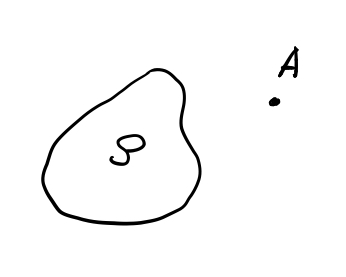
\includegraphics[width=0.4\textwidth]{1_1.jpg}     
 \label{fig:my_label}
 \caption{}
\end{figure}

Посмотрим на рисунок (1.1). Пустьестьнекоторый объем, где плотность заряда $\rho$. Это означает, что в точке \textit{A} поле, создаваемое всем зарядами:

\begin{equation}\label{opr4}
\mathbf{E_{A}} = \int \frac{\rho dV}{r^2} \frac{\mathbf{r}}{|\mathbf{r}|}
\end{equation}

\subsection{Электрический диполь}

\begin{figure}[!ht]
\centering
 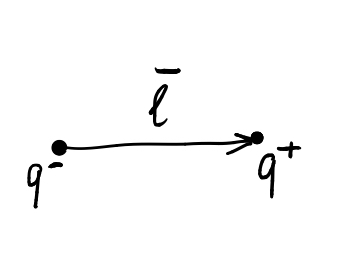
\includegraphics[width=0.4\textwidth]{1_2.jpg}     
 \label{fig:my_label}
 \caption{}
\end{figure}

\colorbox{faded}{\underline{\textbf{Опр.}}} \textbf{Диполь} - это система, состоящая из  двух одинаковых зарядов, одинаковых по величине и противоположных по знаку.

\colorbox{faded}{\underline{\textbf{Опр.}}} \textbf{Плечо диполя $\mathbf{l}$} - вектор, идущий от отрицательного заряда к положительному, длина которого равна расстоянию между зарядами.

\colorbox{faded}{\underline{\textbf{Опр.}}} \textbf{Дипольный момент} - вектор 

\begin{equation}\label{opr5}
\mathbf{p} =q \mathbf{l}
\end{equation}

\begin{figure}[!ht]
\centering
 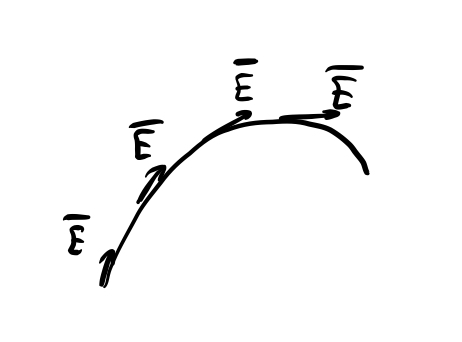
\includegraphics[width=0.4\textwidth]{1_3.jpg}     
 \label{fig:my_label}
 \caption{}
\end{figure}

\colorbox{faded}{\underline{\textbf{Опр.}}} \textbf{Cиловая линия} - линия, в каждой точке которой направление касательной совпадает с направлением напряжённости поля в той же точке. (смотри рис.3)

\colorbox{faded}{\underline{\textbf{Опр.}}} \textbf{Точечный диполь} - диполь, для которого выполнено: расстояние между его зарядами $l$ мало по сравнению с расстоянием $r$ от диполя до точки наблюдения: $l \ll r$

Найдем \underline{поле точечного диполя}:

$$\mathbf{E} = \frac{q}{r^2} \frac{\mathbf{r}}{|\mathbf{r}|} - \frac{q(\mathbf{r} + \mathbf{l})}{|\mathbf{r} + \mathbf{l}|^3}$$

Это выражение разложим в ряд Тейлора (трехмерное разложение):

\begin{equation}\label{opr6}
\mathbf{E} = \frac{3(\mathbf{p} \mathbf{r}) \mathbf{r}}{r^5} - \frac{\mathbf{p}}{r^3}
\end{equation}

\underline{Выведем формулу (6):}

\begin{figure}[!ht]
\centering
 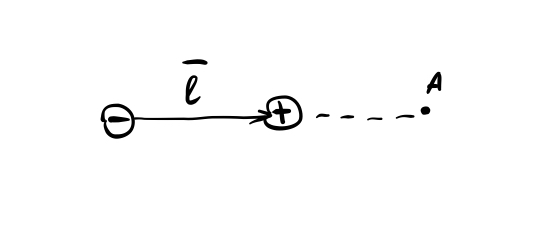
\includegraphics[width=0.4\textwidth]{1_4.jpg}     
 \label{fig:my_label}
 \caption{}
\end{figure}

1. Рассмотрим поле вдоль оси диполя (рисунок 4):
$$E = q \frac{d}{2} (\frac{1}{r^2}) l \Rightarrow \mathbf{E_{||}} = 2 \frac{\mathbf{p}}{r^3}$$

\begin{figure}[!ht]
\centering
 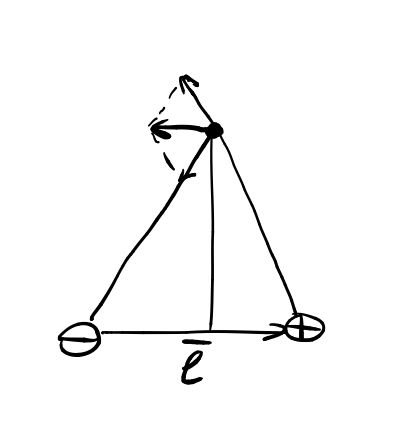
\includegraphics[width=0.4\textwidth]{1_5.jpg}     
 \label{fig:my_label}
 \caption{}
\end{figure}

2. Рассмотрим поле перпендекулярно оси диполя (рисунок 5):
$$\mathbf{E_{\perp}} =  \frac{q}{r^2} \frac{\mathbf{l}}{r}  \Rightarrow \mathbf{E_{\perp}} = - \frac{\mathbf{p}}{r^3}$$

В результате получим (рисунок 6):

\begin{figure}[!ht]
\centering
 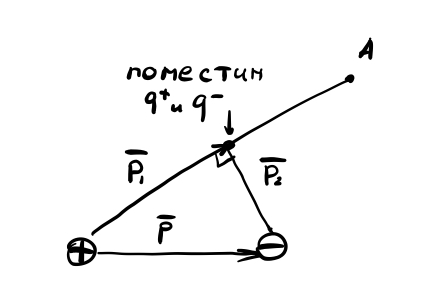
\includegraphics[width=0.4\textwidth]{1_6.jpg}     
 \label{fig:my_label}
 \caption{}
\end{figure}

$$ \mathbf{p}  = \mathbf{p_{1}} + \mathbf{p_{2}}$$
$$\Rightarrow \mathbf{E_{A}} = \frac{2p_{1} - p_{2}}{r^3}$$

Таким образом получили исходное уравнение (6).

\subsection{Демонстрации}

\large
\textbf{\textit{Демонстрация №1.2. "Манка -- это сила!"}}.\\
\normalsize
В данной демонстрации мы увидим диполь. Покажем его с помощью манной крупы. В каждой крупинке под действием ЭП заряды разделяются и каждая крупинка превращается в диполь. На экране видны 2 разноименных заряда. Включим ЭП.
Увидим, что крупинки рисуют силовые линии. 

\large
\textbf{\textit{Демонстрация №1.3. "Султанчики"}}.\\
\normalsize
Зарядим султанчики \underline{одноименно}. Тогда увидим что бумажные полоски расходятся. 
Зарядим султанчики \underline{разноименно}. Тогда увидим что бумажные полоски притягиваются.
\textit{Минутка юмора:} султанчики сходятся до свадьбы, а расходятся после) 

\subsection{Силы, действующие на диполь в ЭП}

\underline{Cлучай 1. $\mathbf{E} = const$}

\begin{figure}[!ht]
\centering
 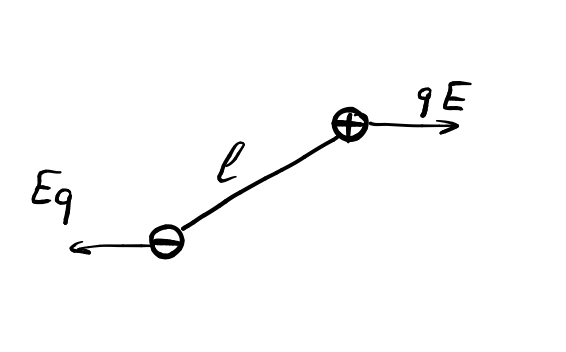
\includegraphics[width=0.4\textwidth]{1_7.jpg}     
 \label{fig:my_label}
 \caption{}
\end{figure}

Поместим диполь в ЭП (рис.7). Силы и напряжение указаны на рисунке. Суммарная сила равно 0, но возникает момент сил:

\begin{equation}\label{opr7}
\mathbf{N} = [\mathbf{l} \mathbf{F}] = [\mathbf{p} \mathbf{E}]
\end{equation}



\underline{Cлучай 2. $\mathbf{E} (\mathbf{r})$}

\begin{equation}\label{opr8}
F = \triangle x \frac{\partial \mathbf{E}}{\partial x} + \triangle y \frac{\partial \mathbf{E}}{\partial y} + \triangle z \frac{\partial \mathbf{E}}{\partial z}
\end{equation}

\colorbox{faded}{\underline{\textbf{Опр.}}} \textbf{Набла}:

\begin{equation}\label{opr9}
\nabla = \mathbf{i}  \frac{\partial}{\partial x} + \mathbf{j} \frac{\partial}{\partial y} + \mathbf{k} \frac{\partial}{\partial z}
\end{equation}

\colorbox{faded}{\underline{\textbf{Опр.}}} Когда оператор набла действует на скалярную функцию - получаем \textbf{градиент $\nabla \Phi$}.

Следовательно, преобразуем формулу (8):
\begin{equation}\label{opr10}
\mathbf{F} = (\mathbf{p} \nabla) \mathbf{E}
\end{equation}

\textbf{Важно:} диполь разворачивается и втягивается в область сильного поля.

\subsection{Теорема Гаусса}

\colorbox{faded}{\underline{\textbf{Опр.}}} \textbf{Поток вектора $d \text{Ф}$}: $d \text{Ф} = \mathbf{E} d \mathbf{S}$ поля \textit{Е} через площадь \textit{S}.

\colorbox{faded}{\underline{\textbf{Теорема Гаусса в интегральной форме}}} Поток вектора \textit{Е} через замкнутую поверхность:

\begin{equation}\label{opr10}
  \oint \mathbf{E} d \mathbf{S} = 4 \pi q
\end{equation}

\underline{\textit{Доказательство:}}

\begin{figure}[!ht]
\centering
 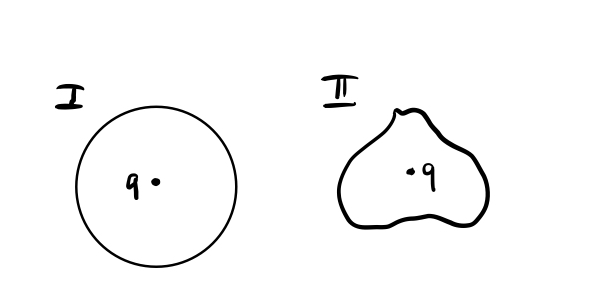
\includegraphics[width=0.4\textwidth]{1_8.jpg}     
 \label{fig:my_label}
 \caption{}
\end{figure}

\underline{Случай 1.} 
$$E = \frac{q}{r^2} \Rightarrow \text{Ф} = 4 \pi r^2 \frac{q}{r^2} = 4 \pi q$$

\underline{Случай 2.} 
$$\oint d \mathbf{S} \mathbf{E} = \oint \frac{q}{r^2}  d S = 4 \pi q
\Rightarrow d \Omega = \frac{\mathbf{r} d \mathbf{S}}{r^3} \text{-- элемент телесного угла}$$

\colorbox{faded}{\underline{\textbf{Теорема Иршоу}}} Невозможна устойчивая статическая конфигурация электрических зарядов
